\documentclass{article}\usepackage[]{graphicx}\usepackage[]{color}
%% maxwidth is the original width if it is less than linewidth
%% otherwise use linewidth (to make sure the graphics do not exceed the margin)
\makeatletter
\def\maxwidth{ %
  \ifdim\Gin@nat@width>\linewidth
    \linewidth
  \else
    \Gin@nat@width
  \fi
}
\makeatother

\definecolor{fgcolor}{rgb}{0.345, 0.345, 0.345}
\newcommand{\hlnum}[1]{\textcolor[rgb]{0.686,0.059,0.569}{#1}}%
\newcommand{\hlstr}[1]{\textcolor[rgb]{0.192,0.494,0.8}{#1}}%
\newcommand{\hlcom}[1]{\textcolor[rgb]{0.678,0.584,0.686}{\textit{#1}}}%
\newcommand{\hlopt}[1]{\textcolor[rgb]{0,0,0}{#1}}%
\newcommand{\hlstd}[1]{\textcolor[rgb]{0.345,0.345,0.345}{#1}}%
\newcommand{\hlkwa}[1]{\textcolor[rgb]{0.161,0.373,0.58}{\textbf{#1}}}%
\newcommand{\hlkwb}[1]{\textcolor[rgb]{0.69,0.353,0.396}{#1}}%
\newcommand{\hlkwc}[1]{\textcolor[rgb]{0.333,0.667,0.333}{#1}}%
\newcommand{\hlkwd}[1]{\textcolor[rgb]{0.737,0.353,0.396}{\textbf{#1}}}%

\usepackage{framed}
\makeatletter
\newenvironment{kframe}{%
 \def\at@end@of@kframe{}%
 \ifinner\ifhmode%
  \def\at@end@of@kframe{\end{minipage}}%
  \begin{minipage}{\columnwidth}%
 \fi\fi%
 \def\FrameCommand##1{\hskip\@totalleftmargin \hskip-\fboxsep
 \colorbox{shadecolor}{##1}\hskip-\fboxsep
     % There is no \\@totalrightmargin, so:
     \hskip-\linewidth \hskip-\@totalleftmargin \hskip\columnwidth}%
 \MakeFramed {\advance\hsize-\width
   \@totalleftmargin\z@ \linewidth\hsize
   \@setminipage}}%
 {\par\unskip\endMakeFramed%
 \at@end@of@kframe}
\makeatother

\definecolor{shadecolor}{rgb}{.97, .97, .97}
\definecolor{messagecolor}{rgb}{0, 0, 0}
\definecolor{warningcolor}{rgb}{1, 0, 1}
\definecolor{errorcolor}{rgb}{1, 0, 0}
\newenvironment{knitrout}{}{} % an empty environment to be redefined in TeX

\usepackage{alltt}
\usepackage{hyperref}
\usepackage{wrapfig}

\title{How can the Santa Ana sucker be saved?}
\author{Marc Los Huertos}
\IfFileExists{upquote.sty}{\usepackage{upquote}}{}
\begin{document}


\maketitle

\section{Introduction}

According to Kolbert 2015, we are in the midst of a dramatic extinction event that is rivaling major catostrophic extinctions in the past. The difference with the current situation is the cause: The dominance of human beings over the Earth's surface led to the extirpation of thousands of species, and counting. 

It's easy to second guess various scientific and policy questions with respect to endangered species, but when we begin to evaluate what is actually being done on the ground for various species, we quickly learn that we are not just in a ecological web, but our policy and regulatory processes are embedded in a complex context of landuse history and economic agendas.  

\begin{wrapfigure}{r}{0.6\textwidth}
  \begin{center}
    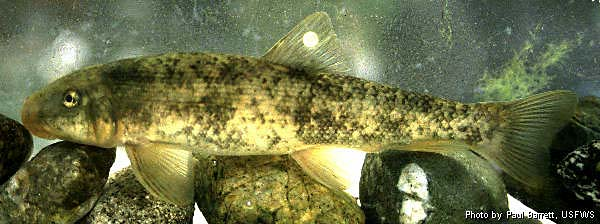
\includegraphics[width=0.58\textwidth]{Catostomus_santaanae.jpg}
  \end{center}
  \caption{Santa Ana sucker, \emph{Catostomus santaanae}}
\end{wrapfigure}

\subsection{Driving Question}

This project will attempt to answer the following question, ``How can we save the Santa Ana sucker?'' As we have seen, this type of generic question needs to be constrained, defined, and subject to what we already know or will learn about the topic. In addition, we need to define the terms used in the question, such as who is "we"? What do we mean by ``save''?  And finally, when we ask ``how'', what are the options avaible that might fit into the ``how''? 

\section{Learing Goals}

\begin{itemize}
  \item Evaluate sucker habitat using the following tools:
  \begin{itemize}
    \item Define Water Quality Goals
    \item Characterize Hydrology and Geomophology
    \item Analyze Community Profile of Periphyton
  \end{itemize}
  \item Propose and evaluate options to improve Santa Ana sucker habitat.
  \item Prepare sets of pratical and effective measures that might protect (or increase) the extant populations of the Santa Ana sucker.
\end{itemize}

\subsection{Why these learning goals?}

\section{Project Stages}

\begin{itemize}
  \item Session 1: Define 'Public Product'
  \item Session 2: Revise 'Driving Question' and list resources needed
  \item Session 3: Read, clarify, or develop appropriate SOPs
  \item Session 4: Field Work
  \item Session 5: Data Analysis
  \item Session 7: Development of Public Products
  \item Session 6: Presentation of Public Products
\end{itemize}

\section{Defining the Public Product}

The stakeholder group has defined the following products for their work:

\begin{description}
  \item[Annoated Bibliography] Thus, we will be collating, organize, and summarize scientific resources that can be digested by a range of stakeholders to help ``answer'' the driving question. 
  \item[Analysis of how invasive red algae affect fish behavior]
  \item[Research Briefs] These briefs will describe the knowledge base, information gaps, and research needs for a range of topics. Each student will contribute one science brief that describes the knowledge available to "resore and protect" the Santa Ana Sucker. Each research brief, will address a different scientific issues associated with the Santa Ana sucker--where each issue addresses a specific driving question with respect to the sucker. EA 30 Research Briefs are short (3-4 pages) descriptions of recently EA30 project results. These ``briefs'' highlights also include one image, a caption (50 words), and several publication citations. Each student will develop one to several briefs that will be made available to the public.
  
Each brief will include 5 sections:

\begin{itemize}
  \item Problem definition
  \item Evidence of problem
  \item Scientific knowledge to address the problem
%  \item Description of Potential Alternative Solutions
  \item Information gaps
  \item Next Steps (which could be translated by stakeholders as potential research needs)
\end{itemize}

  \item[Presentation to HPC on findings] And as the topics develop, we will bundle briefs to produce 3-5 reports that will be made public as part of a presentation to the HPC group.
\end{description}

\subsection{Stakeholders and Evaluation Criteria of Public Product}

Although the audience is the public at large, we will use several collaborators to help us define, refine, and evaluate our public products.  

Our collaborators include: 

\begin{itemize}
  \item USFWS
  \item RCD of SB?
  \item ??
\end{itemize}

west fork...edison... consulting report?



justine...

baskin...(old alheizer..)

annotatee bibl. documents.

recovery permit...

coordinator 10A1A permit...

6-25


980? in carlsbad...

As the develop of individual topics forms, we will form into teams to facilitate field work, literature reviews, and evaluation of current or unpublished data. Hote: each student is responsible for an individual contribution. 

Once we create topical themes, we will create teams to arrange and order of  individual breifs based on the quality and potential interests for each of the sections.  

Working with stakeholders is a key component doing environmental science, which might be constrasted with regular scientific research. Although some make the distinction between applied and pure science, I don't find the divide all that useful. 

Better that getting into the morass of these defintions, let's move on to figure out what skills we need to apply while working with stakeholders. As it turns out, few stakeholders can really define their project until after it is complete -- much to the surprise of the both the stakeholder and the group doing the work. 

There is no secret to get around this problem and even if you identify and try to work through it, you might still find that the project doesn't meet the "expectations" of the stakeholder -- which were either unrealistic or poorly defined or both.

\begin{description}
  \item[Active Listening] Careful listening and echoing what stakeholders say is an extremely important to develop a successful partnership with stakeholders. Asking for clarity and follow up questions will help you define what the goals of the project in collaboration.
  \item[Defining Success] As a key component of collaboration is ensuring that all parties agree on what success look like. For example, this would include examples of "models" to emulate or avoid. In addition, going through the project will help articulate clear expecations about the public product and the workload to get there.
  \item[Outlining a Process] The process can also be called, ``project management''
  \item[Professionalism and Completion]
\end{description}


\begin{wrapfigure}{l}{0.6\textwidth}
   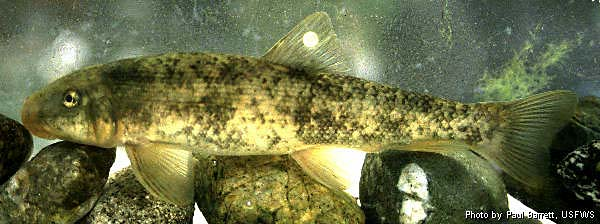
\includegraphics[width=0.58\textwidth]{Catostomus_santaanae.jpg}
  \caption{The Santa Ana sucker \emph{Catostomus santaanae}.}
\end{wrapfigure}

\subsubsection{Kai Pelenscar -- US Fish and Wildlife Service}

\begin{quote}
Based on the current dataset we have on sucker biology and habitat preference, I would like to identify data gaps where student work would contribute to species' conservation as well as contribute to research or other types of projects. In order to prioritize a list of data gaps, I need to know where we stand on the ongoing research projects relating to sucker.

Also, instead of tying the change in habitat to a shutdown, potentially a high velocity flushing flow from RIX [Water treatment facility] would provide data for a measure proposed by Heather's group. 
\end{quote}

\subsubsection{Heather Dyer -- San Bernardino Municipal Water District}

\begin{quote}
I think it would be great to have them [EA30 students] focus on the red algae and its effect on sucker behavior.  

I wonder if we could do a series of snorkel videos of the sucker behavior in/around the red algae (if they are there and utilizing) and compare?

\end{quote}

\subsubsection{Carl Demetropoulos--Fish Ecologists, Consultant}

\begin{quote}
In discussions with other members of the group, we have come along way over the past year and now just need to put it together in a single report, and consider the next phase of analysis.  
\end{quote}

\subsubsection{Larry Brown--USGS}

\begin{quote}
Scott and a colleague have developed a 2-D habitat model of a reach below Rix and Jason works with me on the population estimates and habitat utilization. I am really interested in the dynamics of the red algae below RIX within the modeling reach. This could involve mapping of algae patches and measurements of depth, velocity, and substrate to characterize "algae habitat utilization". This could be compared against sucker habitat utilization to determine if they are "competing" for habitat. Doing this before and several times after a big shutdown would be ideal. This data would be very useful (in my mind anyway) to understanding the sucker population below RIX. I also think this data could contribute to a scientific publication. I was planning on doing this during our fall field work to the extent possible in a week but multiple observations would make for a stronger paper. I think the timing is good since our plan is to do the work in late Sep. The class could overlap or work in Sep-Oct.
\end{quote}

\subsection{US Forest Service -- ??}

forest service... needs some work done too... who is the contact?

\subsection{Southern Edison}


\subsection{Retired--Cam Swift}


\section{Driving Question}

\subsection{Define and constrain driving question}

As one of our first excercises, we will explore the meaning of the driving question. As we work to understand our driving question, we will create groups of students to act as research teams that will address a portion of the driving question.

\subsection{Understanding the Recovery Plan of the Santa Ana sucker}

In the XXX of 20XX, the USFWS release a \href{https://www.fws.gov/carlsbad/SpeciesStatusList/RP/201411xx_Draft%20RP_SASU.pdf}{Draft Recovery Plan for the Santa Ana sucker}. Please read the Draft Plan before class and we will use this to help create the driving question and refine the public product. 

\subsection{Resources to answer driving question}

Each team will determine what resources are avaialble and/or needed to address the driving question. Working with the instructor is key because these resources need to be made available for the following week.

\subsection{Determine Required Resources and Methods}


\subsection{Answering the Driving Questions}




Below is a list of possible themes, but this list in only one potential list and not meant to constrain how we decide to work as a group: 

\begin{description}
  \item[Issue 1: Habitat Use] Where are the Santa Sucker?  Do they move from habitat to habitat on a daily basis? 
  diel movement with a GoPro... successional changes in algae...Video with experimental manipulation of rocks with and without algae on them. E. fork of San Gabriel behavior is much different. More cover...
  
  Select a pool, six pools...too much!  exploratory study.
  
  \item[Issue 2: Food Quality] How has the invassive red algae influenced sucker food? Are diatoms are on the red algae? I
  find a rock and work it up... What about lipid content?  As it turns out that lipid PHA and ARA imputes egg quality upto 3 generations? 
  
  Diatom 18s rDNA
  Faeces 18s rDNA
  
\href{http://www.fao.org/docrep/x5744e/x5744e0f.htm}{http://www.fao.org/docrep/x5744e/x5744e0f.htm}
  
  \item[Issue 3: Water Quality] Temperature, pH, conductivity, DO, and other chemicals?
  \item[Issue 4: Hydrology]Water velocity? flow and feeding behavior... RIX facility...40-100 cfs before and after flushing event..., micro-velocity meter fish my be found in 1.8/2.2 m/s
  \item[Issue 5: Geomorphology] As a comparison, Horse Ranch in Big Tujunga has a 3\% gradient good location/habitat.
\end{description}


\subsection{Data Collection and Analysis}

We will go to the field on three times locations??...

\begin{itemize}
  \item Santa Ana River
  \item San Gabriel River
  \item Big Tujunga Wash
\end{itemize}


?Water Quality

?Velocity








\section{Create Public Product}

To create pubic product, we will develop four/five pdf briefs, using LaTeX and Rstudio. 

\subsection{Selecting a Style}

We will rely on the Tufte style that we can access in Rstudio. 

\subsection{Writing and Presenting Results}

\subsection{Evaluation of the Public Product}

Our stakeholders will evaluate the public product using the criteria that we develop together that will likely include accuracy, scholarship, and clarity. 

\section{Other Resources}

\subsection{Examples}

\href{https://www.fws.gov/Endangered/esa-library/index.html}{https://www.fws.gov/Endangered/esa-library/index.html}

\href{http://blogs.scientificamerican.com/extinction-countdown/}{http://blogs.scientificamerican.com/extinction-countdown/}

\end{document}
